\section{Design architetturale}
%Design architetturale (architettura complessiva, descrizione di pattern architetturali usati, componenti del sistema distribuito, scelte tecnologiche cruciali ai fini architetturali -- corredato da pochi ma efficaci diagrammi)

Di seguito vengono analizzate l'architettura complessiva dell'applicazione e le decisioni critiche riguardanti pattern architetturali e tecnologie rilevanti.
Prima di pensare a qualsiasi architettura per il gioco da realizzare, ciò che si è cercato di fare è stato individuare l'engine ideale per il progetto. 
La scelta è ricaduta su Indigo in quanto: 
\begin{itemize}
    \item E' un framework specifico per il game development
    \item E' scritto in Scala 3 e favorisce lo sviluppo tramite paradigma funzionale con un approccio unidirezionale ed immutabile al flusso di dati
    \item Permette il gioco su browser, come da requisito di business, mediante compilazione tramite Scala.js.
\end{itemize}
I concetti chiave di Indigo che ci guidano nello sviluppo del gioco sono 
\begin{itemize}
    \item Paradigma Model, View, ViewModel
    \item Game loop con modello ad eventi
    \item Scene
\end{itemize}

\subsection{Paradigma Model-View-ViewModel}
Il pattern architetturale \textbf{MVVM} (Model, View, ViewModel) è una variante del famoso MVC. 
Obiettivo di questo pattern è quello di separare il modello dei dati dalla sua rappresentazione, tenendo entrambi puri e funzionali al loro scopo, frapponendo tra loro un elemento "ibrido", il ViewModel.
Di seguito l'interpretazione sulla quale si basa Indigo e che seguiamo per lo sviluppo del nostro gioco.


\begin{figure}[!hbt]
    \centering
    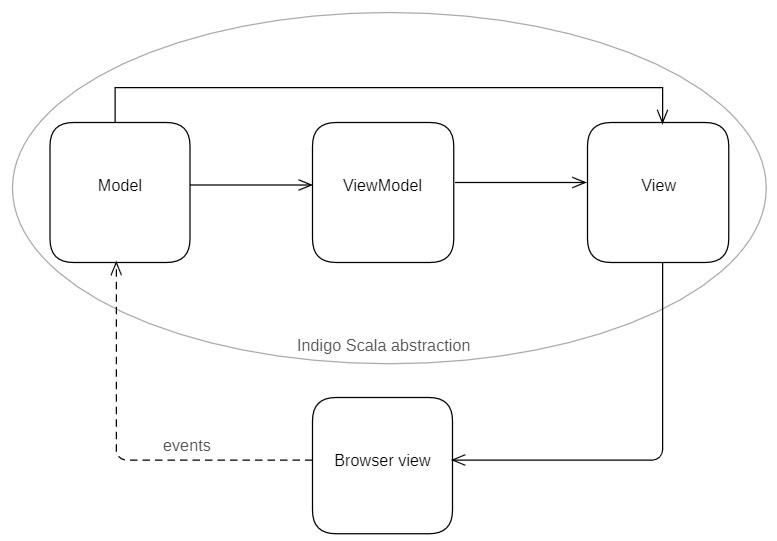
\includegraphics[scale=0.5]{mvvm.jpg}
    \caption{\textit{Architettura Model, View, ViewModel}} 
\end{figure}

\paragraph{Model}
Rappresenta il modello di gioco puro, indipendentemente dalla sua rappresentazione visuale. 
Esso contiene lo stato del gioco e la sua logica. 

\paragraph{ViewModel}
Si interpone tra Model e View. Ha lo scopo di mantenere alcuni dati utili per la rappresentazione che tuttavia non concernono la logica di gioco, devono perciò rimanere separati e non essere inclusi all'interno del Model.

\paragraph{View}
Si occupa di offrire una rappresentazione del Model e del ViewModel a schermo. Costituisce quindi la logica di visualizzazione di questi, senza contenere però alcuno stato o logica di gioco.

\subsection{Game loop con modello ad eventi}
La logica di Indigo si basa su un game loop che processa, ad ogni iterazione, una coda di eventi. 
Ad ogni ciclo, il framework esegue le seguenti operazioni:
\begin{itemize}
    \item Aggiunta dell'evento FrameTick alla coda eventi
    \item Per ogni evento, update del Model
    \item Per ogni evento, update del ViewModel
    \item Presentazione e rendering degli elementi a video
    \item Reset della coda di eventi
\end{itemize}

Il concetto di \textbf{immutabilità}, presente nel paradigma funzionale, qui si traduce non in un update di uno stato interno del modello, ma bensì nella generazione di un nuovo modello aggiornato. 

Durante l'update del Model è possibile generare eventi custom che verranno processati all'iterazione successiva. 

\subsection{Scene}
Le scene sono un modo di organizzare il codice secondo una logica di gioco ben definita. Sono un meccanismo di suddivisione che permette di individuare delle "fasi" di gioco da sviluppare in modo separato le une dalle altre.
In ogni istante all'interno del gioco la scena indicata come "corrente" è abilitata all'aggiornamento del Model/ViewModel, alla gestione degli eventi in coda ed infine alla presentazione a schermo: la scena corrente può leggere e aggiornare solo i suoi dati che sono un sottoinsieme di quelli globali. 

Abbiamo identificato quattro scene principali su cui andare a definire Lost 'n Souls. 

\begin{figure}[!hbt]
    \centering
    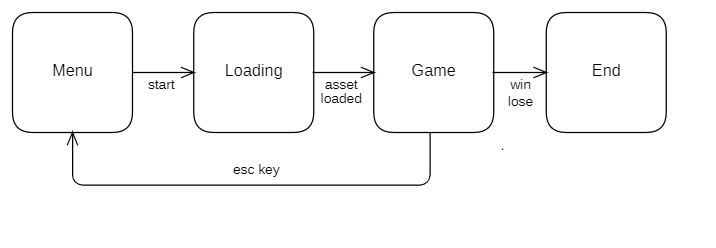
\includegraphics[scale=0.75]{scenes.jpg}
    \caption{\textit{Il flusso delle scene}}
\end{figure}

\subsection{Architettutra di Model e ViewModel}

Come conseguenza della suddivisione di cui sopra, il Model principale è costituito dai singoli Model relativi a ciascuna scena. Stessa cosa vale per il ViewModel. 

Da notare che una scena, per la sua presentazione a video, può non necessitare di un Model o di un ViewModel, lo stesso concetto si può estendere per una View qualsiasi la quale potrebbe basarsi solo su Model.

\begin{figure}[!hbt]
    \centering
    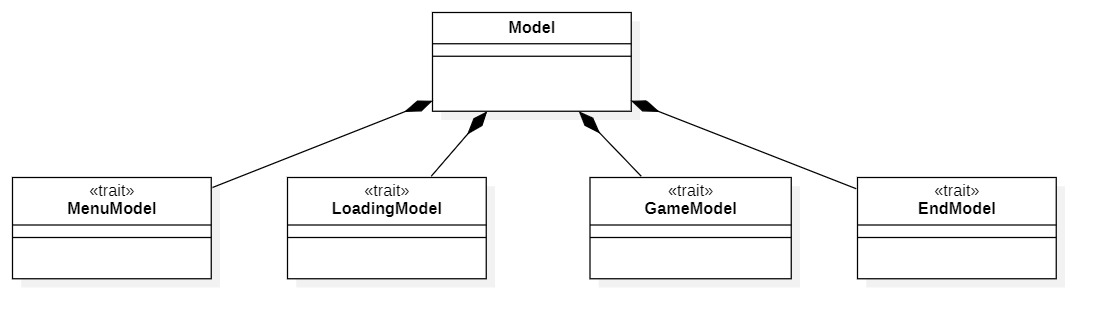
\includegraphics[scale=0.45]{model.jpg}
    \caption{\textit{Il Model}} 
\end{figure}

\newpage 
\subsection{Elementi principali del GameModel}
All'interno della scena di gioco, abbiamo identificato i principali componenti:

\begin{itemize}
    \item \textbf{Character} Personaggio controllato dal giocatore
    \item \textbf{Dungeon} Intera mappa di gioco nel suo complesso
    \item \textbf{Room} Stanza situata all'interno di una mappa di gioco
    \item \textbf{Anything} Una qualsiasi entità da visualizzare all'interno di una stanza: nemico, oggetto, elemento bloccante o anche lo stesso Character. 
    
\end{itemize}


\begin{figure}[!hbt]
    \centering
    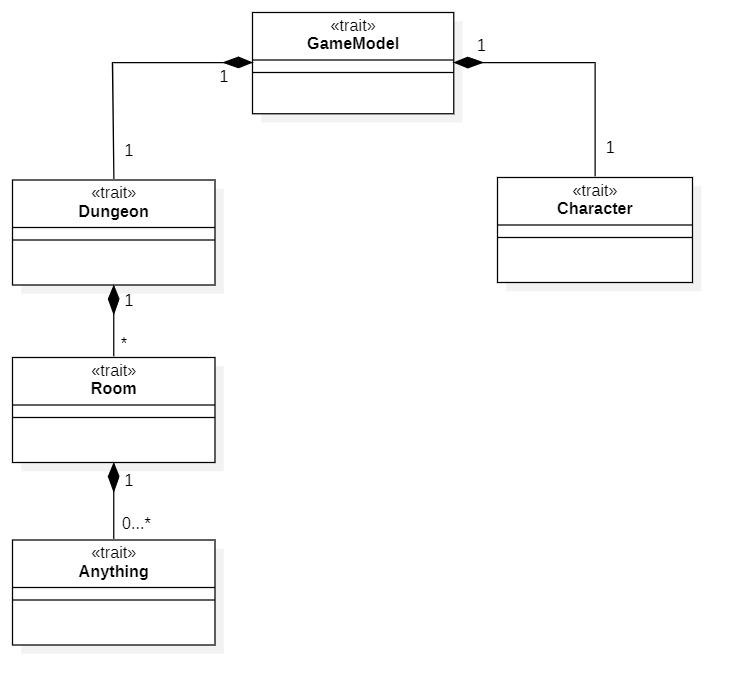
\includegraphics[scale=0.5]{gamemodel.jpg}
    \caption{\textit{Diagramma degli elementi principali del GameModel}} 
\end{figure}

\subsection{Anything OOP anziché pattern ECS}
Per concludere la descrizione dell'architettura occorre specificare come organizzare gli oggetti presenti nel gioco, quelli che abbiamo chiamato \textbf{Anything}.
Un oggetto è caratterizzato da proprietà e comportamenti comuni ad altri, ad esempio tutti gli oggetti sono posizionabili nella stanza di gioco e visualizzabili mentre alcuni di questi possono spostarsi, collidere, causare danno e così via.

Tradizionalmente molto usato nel game development è il pattern Entities-Components-Systems che prevede la sostituzione di una gerarchia di oggetti con il concetto di entità e componenti: le entità sono definite dai diversi componenti a loro associati. 
Alcune implementazioni di ECS definiscono i componenti come solo strutture dati mentre il comportamento è specificato nel sistema che li gestisce, quindi in stile funzionale. 
Questo pattern è nato per diversi motivi ma quello più banale è che, quando i linguaggi non supportano l'ereditarietà multipla, è impossibile specificare una precisa gerarchia di oggetti che soddisfi i requisiti di un gioco di una certa complessità, o comunque questa gerarchia sarebbe molto profonda e poco flessibile a future estensioni.

Quello che vogliamo fare in questo progetto è sfruttare appieno le potenzialità in ambito \textbf{OOP} che ci offre Scala, il quale ci permette tramite i \textbf{mix-ins} di appiattire la gerarchia ed ottenere la flessibilità richiesta dal problema.
Quindi abbiamo appositamente scelto il nome Anything in sostituzione al classico Entity per specificare che non stiamo applicando il pattern ECS, un sottotipo di Anything rappresenta una nostra entità che può essere mixata con altri tratti per ottenere nuove proprietà e comportamenti. 

Visto l'impiego del pattern MVVM, occorre inoltre tenere ben presente che un Anything deve essere in realtà codificato in tre parti ben distinte Model-ViewModel-View ciascuna sottotipo rispettivamente di \textbf{AnythingModel}, \textbf{AnythingViewModel} e \textbf{AnythingView} e ciascuna eventualmente mixata come descritto precedentemente. 
Inoltre è da specificare che ogni oggetto in gioco è costitutito sempre da un Model e una View ma quest'ultima potrebbe non necessitare di un ViewModel.

Il Model di un oggetto come comportamento base deve reagire alle richieste di aggiornamento che avvengono ad ogni iterazione del game loop: questa richiesta deve essere propagata a tutta la catena di ereditarietà e ai vari oggetti mixati ed infine restituire un nuovo Model aggiornato.
Sebbene gran parte del comportamento e della logica di gioco è così incapsulata nei Model degli oggetti, dovremmo comunque elaborare dei sistemi che avranno una visione globale gestendo l'interazione tra diversi Model, come un sistema per controllare le collisioni tra oggetti.

Per concludere, la nostra soluzione OO non è la migliore soluzione possibile per lo sviluppo di un gioco. Il pattern ECS ha vantaggi prestazionali riconosciuti sia in termini di utilizzo CPU (meno calls per l'aggiornamento degli oggetti) che di ottimizzazione dell'utilizzo della memoria (data-oriented design), tuttavia a fini didattici vogliamo sperimentare elementi di Scala OOP avanzati.

\subsection{Prolog engine e PrologService}
Il motore Prolog da utilizzare per la generazione del dungeon, delle stanze combattimento e del comportamento del Boss deve potersi integrare ed interagire con Indigo.
Poichè Indigo compila con Scala.js e per evitare possibili problemi con engine scritti in Java/Scala, la scelta di quale motore Prolog usare ricade su \textbf{TauProlog}, un engine scritto in Javascript e quindi facilmente integrabile nel nostro contesto.

Tuttavia per comunicare con questo motore occorre utilizzare la \textbf{programmazione asincrona} in quanto è strutturato in modo da rispondere alle interrogazioni mediante una \textbf{callback} che deve essere fornita.
Questa modalità di interazione non è supportata direttamente da Indigo, il quale con il suo game loop supporta come input eventi/messaggi che però possono essere generati solo internamente durante le fasi di update del Model: l'attivazione di una callback asyncrona fuori dal game loop non può ne modificare lo stato del Model che è immutabile ne generare un evento.

Per questo si rende necessario lo sviluppo di un componente separato che faccia da proxy per l'engine TauProlog e risponda alle richieste del gioco con opportuni eventi customizzati.

Indigo dispone dei \textbf{SubSystems}, servizi con un proprio Model ed esterni alla logica di gioco ma che vengono attivati nel game loop per intercettare eventi ed eseguire azioni: occorre quindi predispore un \textbf{PrologService} subsystem.

\begin{figure}[!hbt]
    \centering
    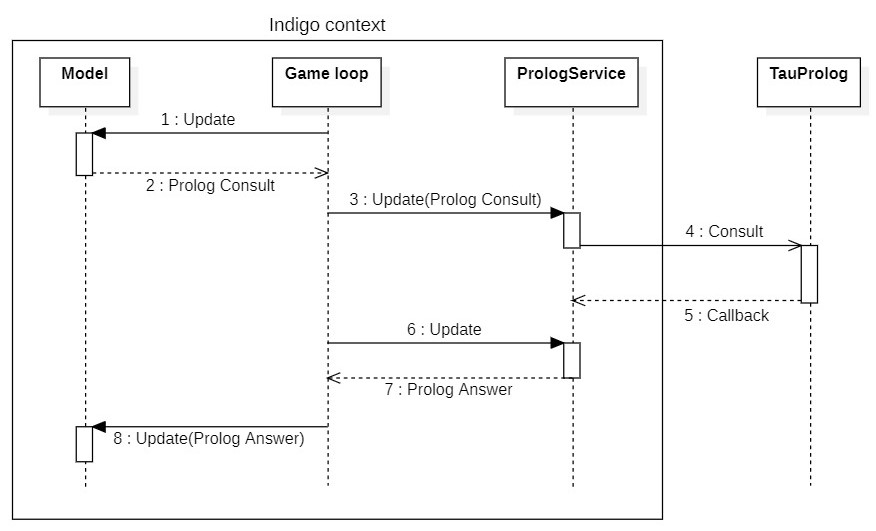
\includegraphics[scale=0.7]{prolog.jpg}
    \caption{\textit{Diagramma dell'interazione con TauProlog}} 
\end{figure}

In figura sotto è mostrata l'interazione tra i sistemi: da notare che la callback chiamata da TauProlog necessita di scrivere dati nel Model del PrologService invalidando così il concetto di immutabilità, ma solo per quel servizio esterno al gioco ed il tutto senza introdurre alcun problema di concorrenza in quanto ogni esecuzione di procedura è atomica nel contesto dell'\textbf{event loop} di Javascript.


